\documentclass[12pt,a4paper]{book}
\usepackage{lmodern}
\usepackage{amssymb,amsmath}
\usepackage{ifxetex,ifluatex}
\usepackage{fixltx2e} % provides \textsubscript
\ifnum 0\ifxetex 1\fi\ifluatex 1\fi=0 % if pdftex
  \usepackage[T1]{fontenc}
  \usepackage[utf8]{inputenc}
\else % if luatex or xelatex
  \ifxetex
    \usepackage{mathspec}
  \else
    \usepackage{fontspec}
  \fi
  \defaultfontfeatures{Ligatures=TeX,Scale=MatchLowercase}
\fi
% use upquote if available, for straight quotes in verbatim environments
\IfFileExists{upquote.sty}{\usepackage{upquote}}{}
% use microtype if available
\IfFileExists{microtype.sty}{%
\usepackage{microtype}
\UseMicrotypeSet[protrusion]{basicmath} % disable protrusion for tt fonts
}{}
\usepackage[margin=1in]{geometry}
\usepackage{hyperref}
\hypersetup{unicode=true,
            pdfborder={0 0 0},
            breaklinks=true}
\urlstyle{same}  % don't use monospace font for urls
\usepackage{natbib}
\bibliographystyle{plainnat}
\usepackage{longtable,booktabs}
\usepackage{graphicx,grffile}
\makeatletter
\def\maxwidth{\ifdim\Gin@nat@width>\linewidth\linewidth\else\Gin@nat@width\fi}
\def\maxheight{\ifdim\Gin@nat@height>\textheight\textheight\else\Gin@nat@height\fi}
\makeatother
% Scale images if necessary, so that they will not overflow the page
% margins by default, and it is still possible to overwrite the defaults
% using explicit options in \includegraphics[width, height, ...]{}
\setkeys{Gin}{width=\maxwidth,height=\maxheight,keepaspectratio}
\IfFileExists{parskip.sty}{%
\usepackage{parskip}
}{% else
\setlength{\parindent}{0pt}
\setlength{\parskip}{6pt plus 2pt minus 1pt}
}
\setlength{\emergencystretch}{3em}  % prevent overfull lines
\providecommand{\tightlist}{%
  \setlength{\itemsep}{0pt}\setlength{\parskip}{0pt}}
\setcounter{secnumdepth}{5}
% Redefines (sub)paragraphs to behave more like sections
\ifx\paragraph\undefined\else
\let\oldparagraph\paragraph
\renewcommand{\paragraph}[1]{\oldparagraph{#1}\mbox{}}
\fi
\ifx\subparagraph\undefined\else
\let\oldsubparagraph\subparagraph
\renewcommand{\subparagraph}[1]{\oldsubparagraph{#1}\mbox{}}
\fi

%%% Use protect on footnotes to avoid problems with footnotes in titles
\let\rmarkdownfootnote\footnote%
\def\footnote{\protect\rmarkdownfootnote}

%%% Change title format to be more compact
\usepackage{titling}

% Create subtitle command for use in maketitle
\newcommand{\subtitle}[1]{
  \posttitle{
    \begin{center}\large#1\end{center}
    }
}

\setlength{\droptitle}{-2em}
  \title{\textbf{\LARGE R을 이용한 자료처리 및 시각화}}
  \pretitle{\vspace{\droptitle}\centering\huge}
  \posttitle{\par}
\subtitle{\textbf{\Large 기본 환경 설정부터 재현가능한 연구 방법 입문}\vspace{2cm}\linebreak 한국한의학연구원
한의기반연구부\linebreak Korea Institute of Oriental Medicine, KM
Fundamental Research Division \vspace{2cm}}
  \author{\textbf{\Large 구본초, Ph.D. in Statistics}}
  \preauthor{\centering\large\emph}
  \postauthor{\par}
  \predate{\centering\large\emph}
  \postdate{\par}
  \date{2017-11-23}

\usepackage{kotex}
\usepackage{placeins}
\usepackage{enumerate}

\usepackage{setspace}\doublespacing
\usepackage{relsize}
\usepackage{bigints}
\usepackage{bm}
\usepackage{lipsum}
\usepackage{booktabs}
\usepackage{dcolumn}
\usepackage{array}
\usepackage[font=small,labelfont=bf]{caption}
\usepackage{gensymb}
\usepackage{makecell}
\usepackage{multirow}
\usepackage{natbib}
\usepackage{threeparttable}
\usepackage{rotating}
\usepackage[table]{xcolor}
\usepackage{graphicx,grffile}

\renewcommand\theadalign{cb}
\renewcommand\theadfont{\bfseries}
\renewcommand\theadgape{\Gape[4pt]}
\renewcommand\cellgape{\Gape[4pt]}
\DeclareMathAlphabet{\mathpzc}{OT1}{pzc}{m}{it}

\renewcommand\theadalign{cb}
\renewcommand\theadfont{\bfseries}
\renewcommand\theadgape{\Gape[4pt]}
\renewcommand\cellgape{\Gape[4pt]}

\newcolumntype{L}[1]{>{\raggedright\let\newline\\
\arraybackslash\hspace{0pt}}m{#1}}
\newcolumntype{C}[1]{>{\centering\let\newline\\
\arraybackslash\hspace{0pt}}m{#1}}
\newcolumntype{R}[1]{>{\raggedleft\let\newline\\
\arraybackslash\hspace{0pt}}m{#1}}
\newcolumntype{P}[1]{>{\raggedright\tabularxbackslash}p{#1}}
\newcommand{\specialcell}[2][c]{%
  \begin{tabular}[#1]{@{}c@{}}#2\end{tabular}}
\newcommand{\specialcelll}[2][l]{%
  \begin{tabular}[#1]{@{}l@{}}#2\end{tabular}}


\captionsetup[table]{aboveskip=0pt}
\captionsetup[table]{belowskip=10pt}

\pagestyle{plain}
% \linespread{1.5}

\begin{document}
\maketitle

{
\setcounter{tocdepth}{1}
\tableofcontents
}
\chapter{R을 사용하기 위한 환경 설정}\label{r----}

\section{Overview}\label{overview}

\subsection{What is R?}\label{what-is-r}

\begin{itemize}
\item
  R 언어: 통계 및 자료 시각화를 지원하는 언어 및 환경
\item
  1980년 AT\&T 연구소의 John Chambers가 개발한 S 언어를 기반으로 1995년
  뉴질랜드 Auckland Univ.의 Robert Gentleman \& Ross Ihaka 개발이 그
  기원임
\item
  GNU 기반 오픈소스
\end{itemize}

\subsection{Why R?}\label{why-r}

\begin{enumerate}
\def\labelenumi{\arabic{enumi}.}
\tightlist
\item
  장점

  \begin{itemize}
  \tightlist
  \item
    \textbf{Free software}
  \item
    주요 운영체제(Unix, Windows, Macintosh)에서 사용 가능
  \item
    현존하는 거의 대부분의 통계 방법론들이 package로 구현
  \item
    강력한 그래픽 기능
  \item
    빠른 update 및 연산속도(?)
  \item
    방대한 community 및 R package에 공개 및 공유된 자료
  \end{itemize}
\item
  Do we have to learn R language?

  \begin{itemize}
  \tightlist
  \item
    물론 꼭 배울 필요는 없다!! (요리를 하는데 꼭 좋은 칼이 필요
    없듯이\ldots{})
  \item
    다양한 통계 소프트웨어 및 분석 언어(SPSS, SAS, WEKA, MATLAB, PYTHON,
    \ldots{}) 존재
  \item
    프로그래밍에 익숙하지 않은 사용자들의 접근성이 떨어짐
  \item
    하지만 배워두면 좋은 이유

    \begin{itemize}
    \tightlist
    \item
      통계분석과 보고서 작성을 위한 최적 환경

      \begin{itemize}
      \tightlist
      \item
        R + Rstudio + Rmarkdown을 통해 분석에서부터 보고서 작성까지
        한번에 가능
      \end{itemize}
    \item
      SPSS, SAS에 비해 확장성이 높기 때문에 다양한 문제에 적용 가능
    \item
      방대한 양의 메뉴얼 및 서적들
    \item
      그리고 이 모든 것을 거의 대부분 무료 사용 가능
    \end{itemize}
  \end{itemize}
\end{enumerate}

\begin{quote}
\colorbox{gray!10}{\begin{minipage}{15cm}
\textbf{Tips}
  \begin{itemize}
    \item R에서 구현한 모든 package들은 CRAN (The Comprehensive R Archive Network, http://cran.r-project.org/web/view)에서 살펴볼 수 있음
    \item R과 관련한 대부분의 문제는 Google 검색과 스텍 오버플로우(http://stackoverflow.com)에서 해결할 수 있음
    \item 본 문서는 서민구 선생님의 ``R을 이용한 데이터 처리 \& 실무'' \citep{Seo-2014} 와 고석범 선생님의 ``R과 Knitr을 활용한 데이터 연동형 문서 만들기'' \citep{Ko-2014} 의 내용을 주로 참조함. 
  \end{itemize}
\end{minipage}}
\end{quote}

\newpage

\section{R 설치하기(Windows 용)}\label{r-windows-}

R은 공개 소프트웨어로 \url{http://www.r-project.org/} 에서 다운로드 및
설치 가능

\begin{enumerate}
\def\labelenumi{\arabic{enumi}.}
\tightlist
\item
  웹브라우저(i.e.~explore, chrome, firefox 등)에서
  \url{http://www.r-project.org} 이동
\item
  좌측 R Logo 하단 Download 아래 `CRAN' 클릭
\end{enumerate}

\begin{figure}[h]
{
  \centering
  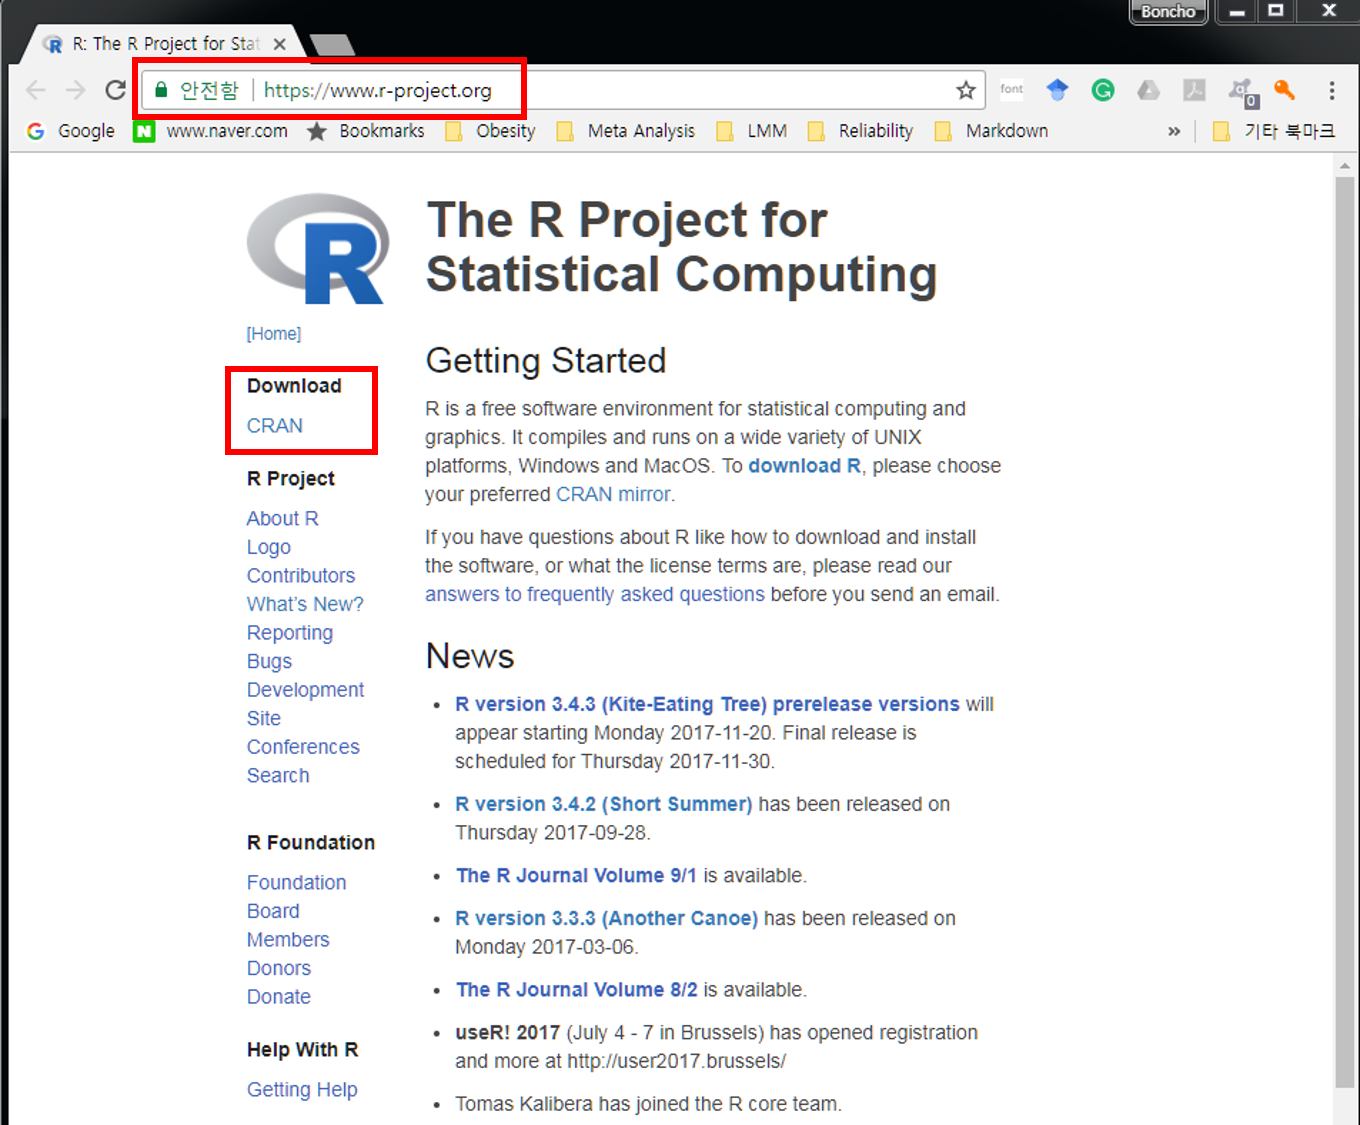
\includegraphics[width = 12cm, height = 12cm]{Figures/Rorg-main-add.png}
  \caption[www.r-project.org 메인화면]{www.r-project.org 메인화면}\label{fig:R-install-01}
}
\end{figure}

\begin{enumerate}
\def\labelenumi{\arabic{enumi}.}
\setcounter{enumi}{2}
\tightlist
\item
  클릭 후 연결 창에서 스크롤 후 ``Korea'' 아래 링크 클릭 (그림
  \ref{fig:R-install-02} 참조)
\end{enumerate}

\begin{figure}[h]
{
  \centering
  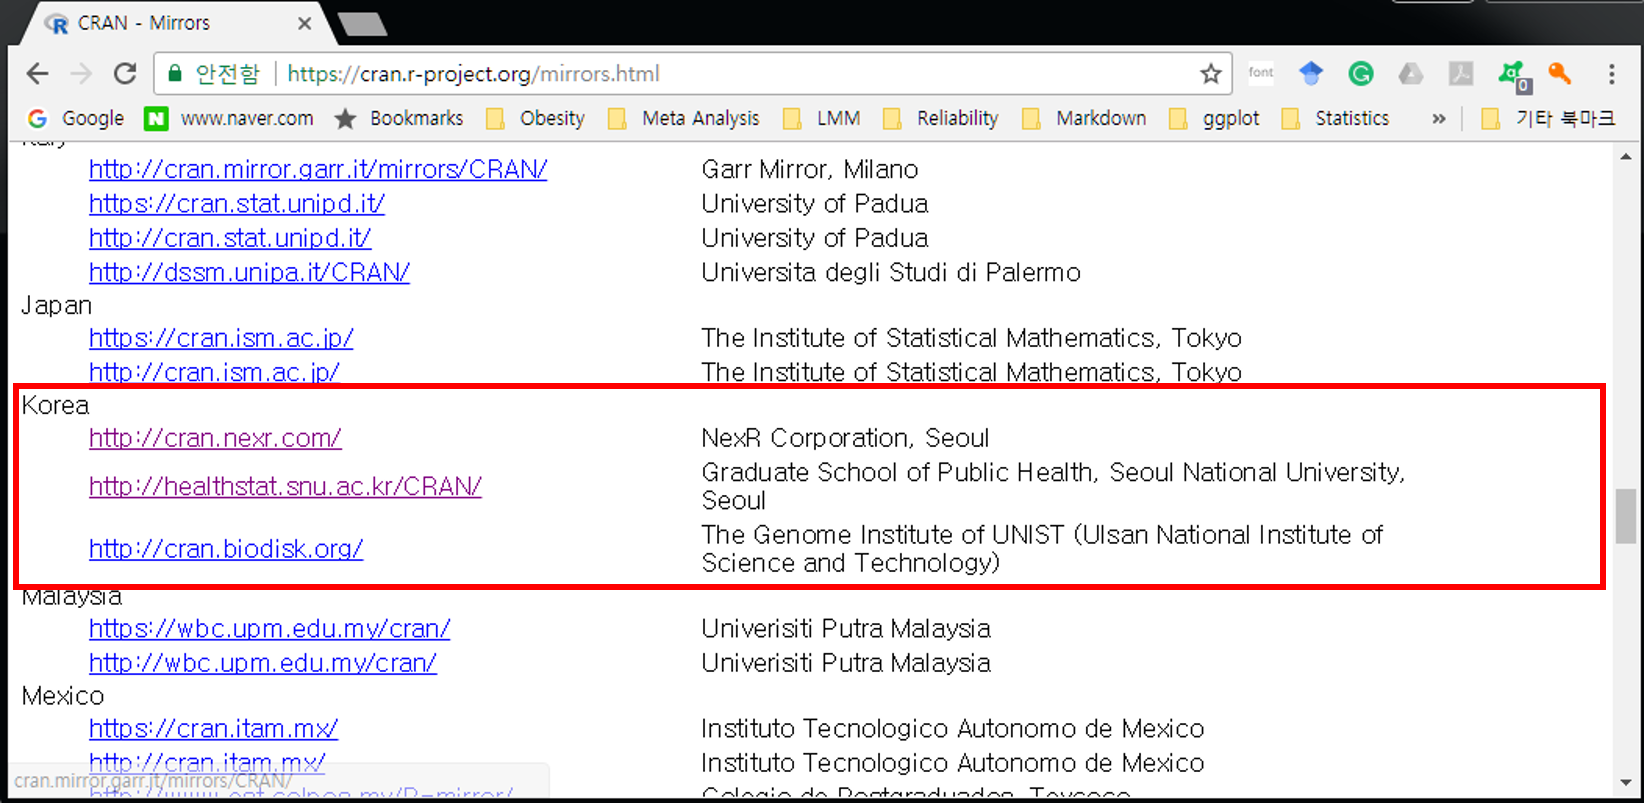
\includegraphics[width = 12cm, height = 8cm]{Figures/CRAN-korea-01.PNG}
  \caption[CRAN 국가별 mirrors]{CRAN 국가별 mirrors}\label{fig:R-install-02}
}
\end{figure}

\begin{enumerate}
\def\labelenumi{\arabic{enumi}.}
\setcounter{enumi}{3}
\tightlist
\item
  클릭 후 세 가지 운영체제(Linux, Mac OS X, Windowns)에 따른 R 버전 선택
  가능

  \begin{itemize}
  \tightlist
  \item
    본 문서에서는 Windows 버전 설치만 다룸
  \end{itemize}
\end{enumerate}

\begin{figure}[h]
{
  \centering
  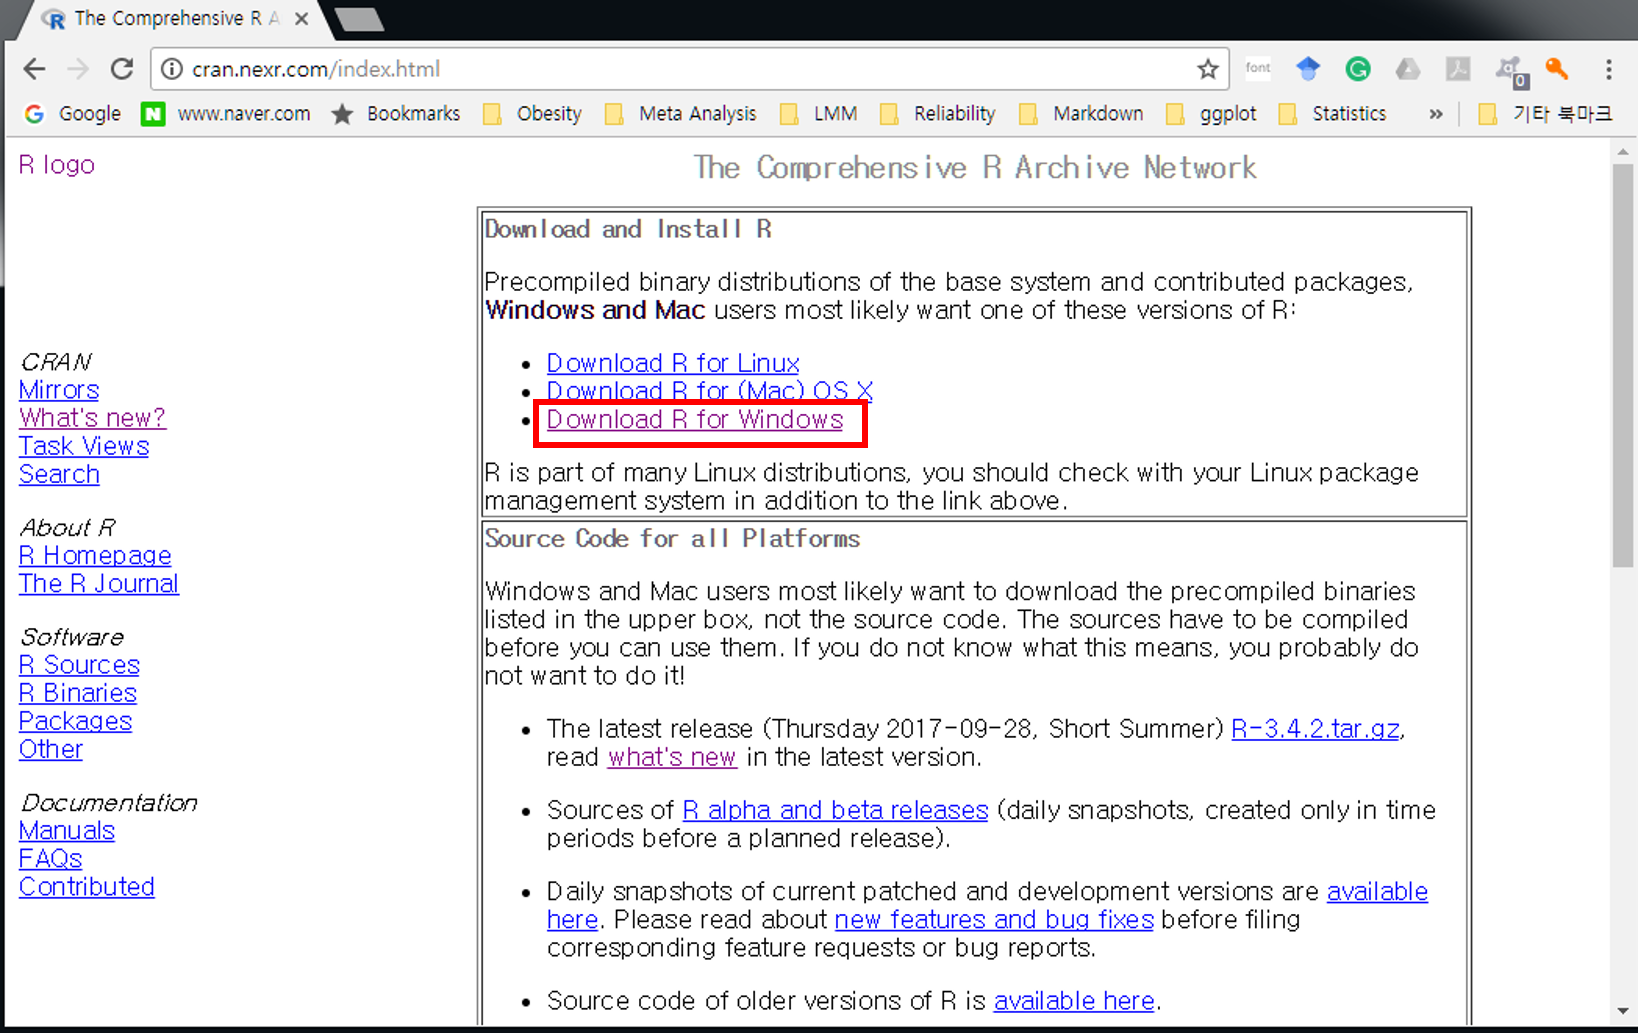
\includegraphics[width = 12cm, height = 10cm]{Figures/Rinstall-01.png}
  \caption[운영체제 별 R 버전 선택]{운영체제 별 R 버전 선택}\label{fig:R-install-03}
}
\end{figure}

\begin{enumerate}
\def\labelenumi{\arabic{enumi}.}
\setcounter{enumi}{4}
\tightlist
\item
  ``Downloads R for Windows'' 링크 클릭하면 다음과 같은 화면으로 이동
\end{enumerate}

\begin{figure}[h]
{
  \centering
  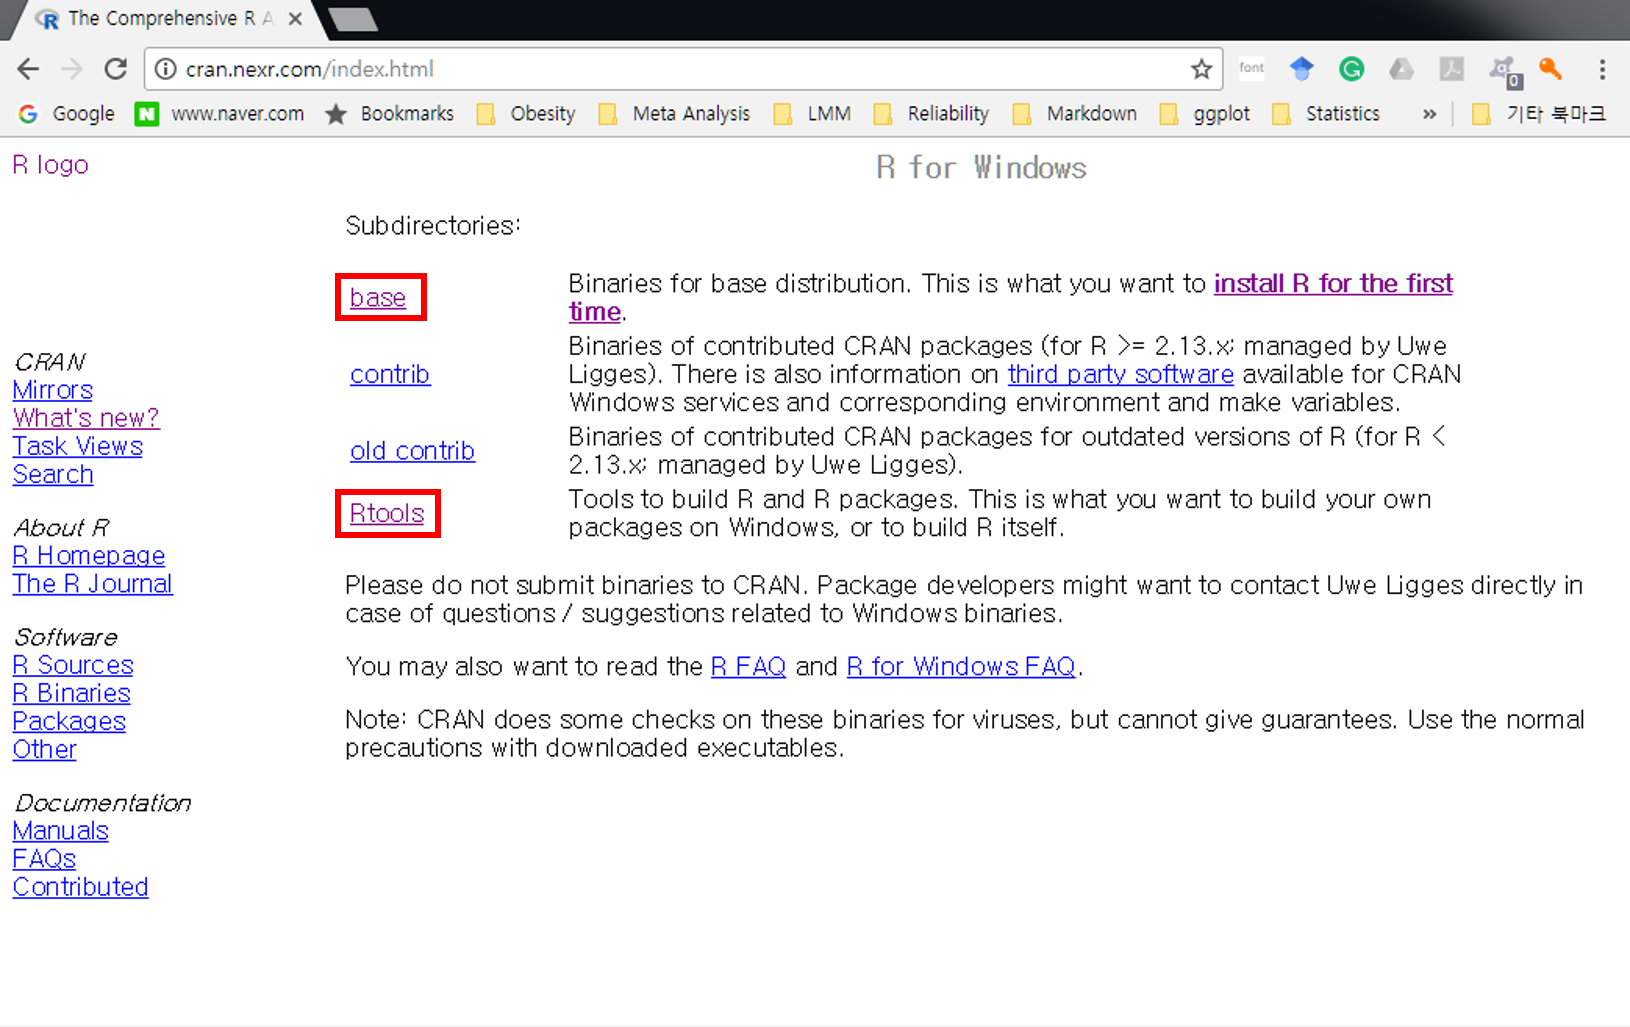
\includegraphics[width = 12cm, height = 10cm]{Figures/Rinstall-02.png}
  \caption[Windows 용 R base 및 구성요소 다운로드]{Windows 용 R base 및 구성요소 다운로드}\label{fig:R-install-04}
}
\end{figure}

\begin{enumerate}
\def\labelenumi{\arabic{enumi}.}
\setcounter{enumi}{5}
\item
  R을 구성하는 하위구조 중 ``base'' 링크 클릭 후 다음 화면에서
  ``Downloads R 3.4.2 for Windows''를 클릭 후 설치 파일을 임의의
  디렉토리에 저장 후 실행(그림 \ref{fig:R-install-05} 참조)
\item
  참고로 3개 subdirectories에 대한 간략한 설명은 아래와 같음

  \begin{itemize}
  \tightlist
  \item
    \texttt{base}: R 실행 프로그램
  \item
    \texttt{contrib}: R package의 바이너리 파일
  \item
    \texttt{Rtools}: R package 개발 및 배포를 위한 프로그램
  \end{itemize}
\end{enumerate}

\begin{figure}[h]
{
  \centering
  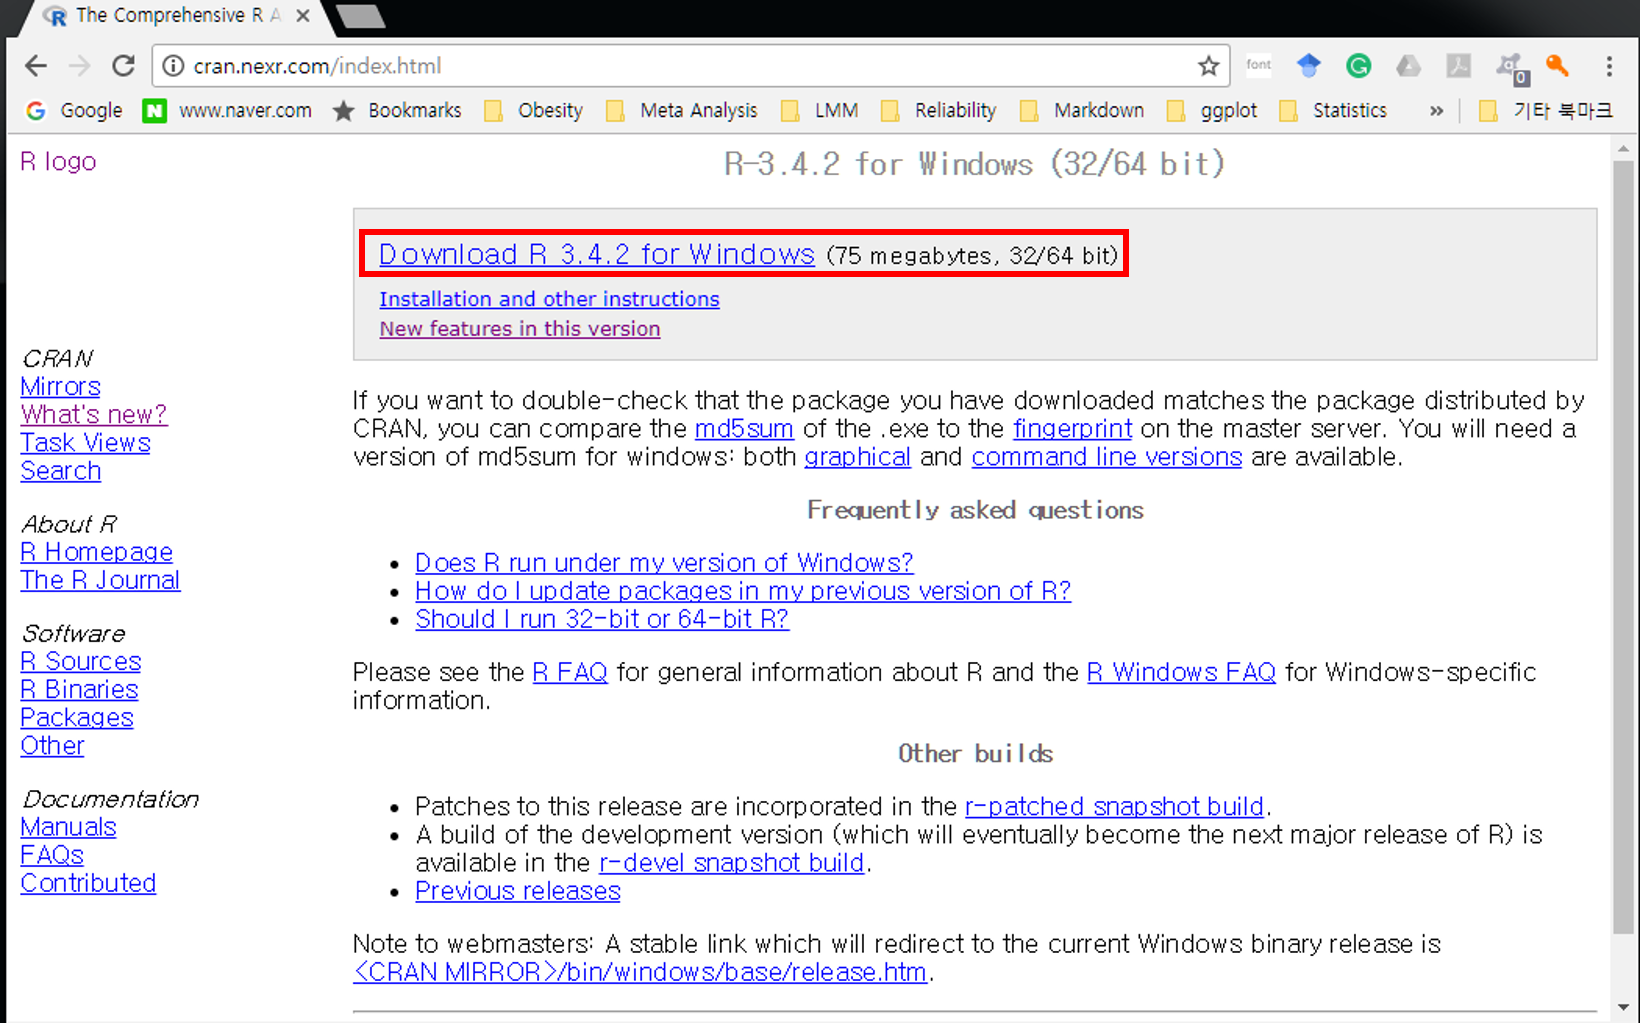
\includegraphics[width = 12cm, height = 10cm]{Figures/Rinstall-03.png}
  \caption[Windows 용 R 설치 파일 다운로드 페이지]{Windows 용 R 설치 파일 다운로드 페이지}\label{fig:R-install-05}
}
\end{figure}

\begin{enumerate}
\def\labelenumi{\arabic{enumi}.}
\setcounter{enumi}{7}
\tightlist
\item
  다운로드한 파일을 실행하면 아래와 같은 대화창이 나타남

  \begin{itemize}
  \tightlist
  \item
    한국어 선택 \(\rightarrow\) 환영 화면에서
    {[}다음(N)\textgreater{}{]} 클릭
  \end{itemize}
\end{enumerate}

\begin{figure}[h]
{
  \centering
  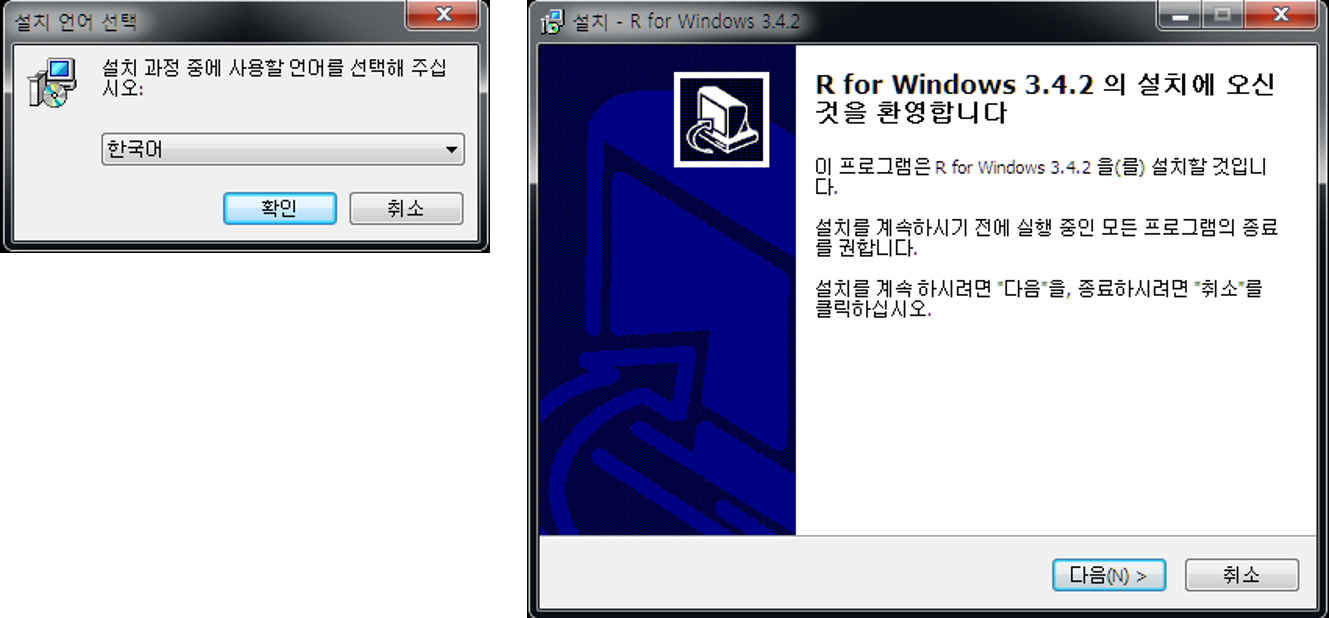
\includegraphics[width = 14cm, height = 11cm]{Figures/R-install-F01.png}
  \caption[R 설치과정 01]{R 설치과정 01}\label{fig:R-install-06}
}
\end{figure}

\begin{enumerate}
\def\labelenumi{\arabic{enumi}.}
\setcounter{enumi}{8}
\tightlist
\item
  GNU 라이센스에 대한 설명 및 동의 여부({[}다음(N)\textgreater{}{]})
  클릭 (그림 \ref{fig:R-install-07})
\end{enumerate}

\begin{figure}[h]
{
  \centering
  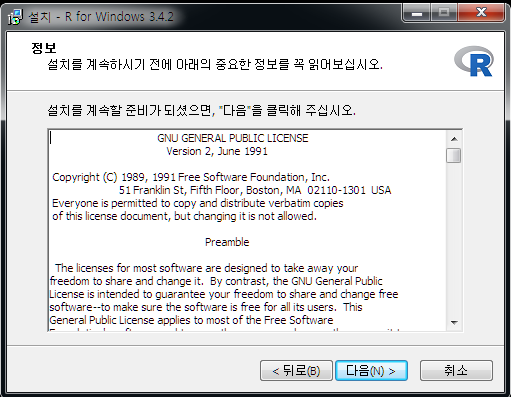
\includegraphics[width = 10cm, height = 10cm]{Figures/R-install-F02.png}
  \caption[R GNU general license]{R GNU general license}\label{fig:R-install-07}
}
\end{figure}

\begin{enumerate}
\def\labelenumi{\arabic{enumi}.}
\setcounter{enumi}{9}
\tightlist
\item
  설치 디렉토리 설정 및 구성요소 설지 여부

  \begin{itemize}
  \tightlist
  \item
    원하는 디렉토리 설정(예:
    \texttt{C:\textbackslash{}R\textbackslash{}R-3.4.2})
  \item
    기본 프로그램 및 32 또는 64 bit 용 설치 파일, R console 한글 번역
    모두 체크 뒤 {[}다음(N)\textgreater{}{]} 클릭
  \end{itemize}
\end{enumerate}

\begin{figure}[h]
{
  \centering
  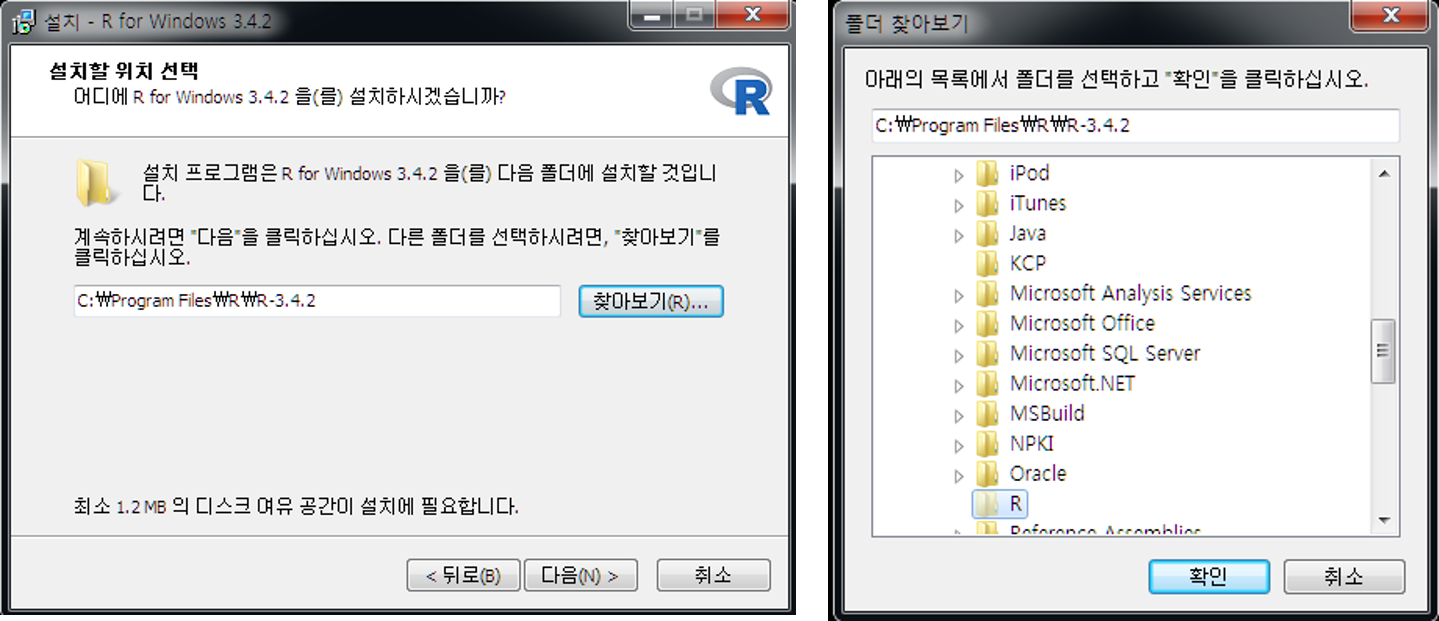
\includegraphics[width = 15cm, height = 10cm]{Figures/R-install-F03.png}
  \caption[R 설치 디렉토리 설정]{R 설치 디렉토리 설정}\label{fig:R-install-08}
}
\end{figure}

\renewcommand\bibname{References}
\bibliography{CNUH.bib}


\end{document}
